\chapter{Older Adults and Their Attitudes Towards Exercising}
\label{chap:olderexercise}
Physical activity is important for all people, including elderly. It can improve quality of life by reducing risk of some chronic diseases, alleviate depression, and help people towards a more independent life. Improving health by physical activity does not just apply for healthy elderly, but also for frail and very old people. Guidelines are proposed by the Department of Health and Human Services, recommending aerobic activity, as well as muscle-strength training \cite{guidelines}. These guidelines  may seem easy to follow, but it is shown to be challenging to motivate elderly to exercise, and there is shown that there is a small percentage of elderly who actually engage in physical activity \cite{olderamericans}. To be able to engage seniors to be more physically active, they should be provided with programs that will motivate them to actually perform the exercises. In this thesis, we will develop a game concept for this purpose. This game have to have the right elements in place, to motivate the user to engage in regular physical activity. (It needs to relate to their life, and it needs to be offered at placed where they can actually use it.) As discussed in our previous project \cite{project} and in \cite{schutzer}, keeping the older population healthy, can in addition to reduce the need for health services, also decrease economic challenges related to this.  It is therefore important to have focus on elderly's physical health. 

\begin{figure}
\begin{center}
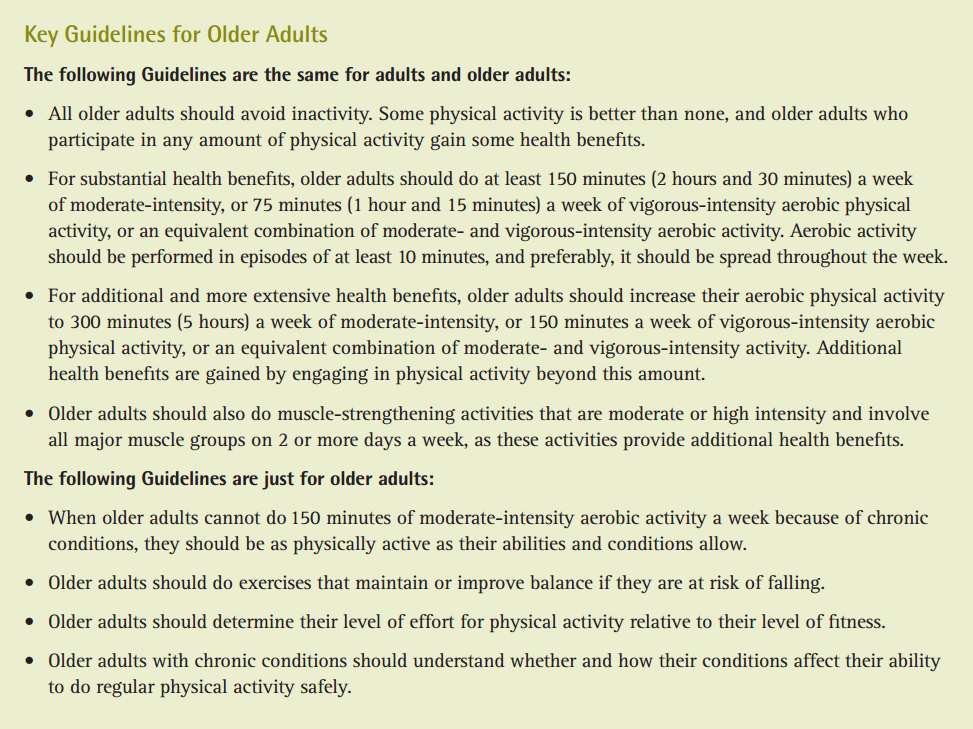
\includegraphics[scale=0.5]{exercisegl}
\caption[Physical activity guidelines for older adults]{Physical activity guidelines for older adults \cite{guidelines}}
\label{fig:exercisegl}
\end{center}
\end{figure} 

\begin{figure}
\begin{center}
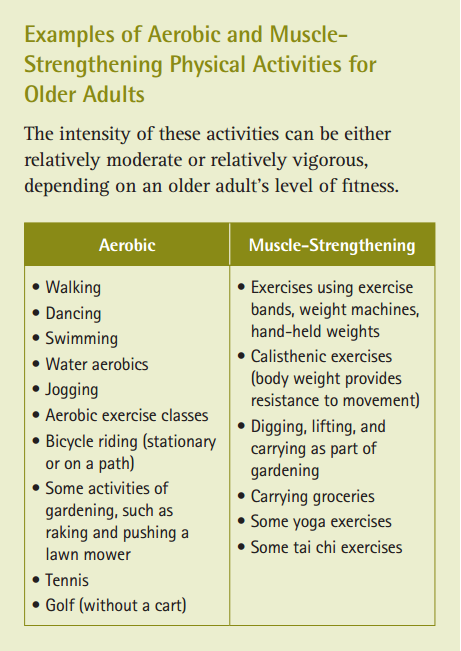
\includegraphics[scale=0.6]{typeofexercise}
\caption[Examples of aerobic and muscle-strengthening physical activities for 
older adults ]{Examples of aerobic and muscle-strengthening physical activities for 
older adults \cite{guidelines}}
\label{fig:typeofexercise}
\end{center}
\end{figure} 

Norwegian elderly, aged  67-79 years old, have actually become more active the last years, with as much as 40 percent of this population exercising regularly several times a week \cite{statisticsnorway}. Whether they meet the requirements of how much they should exercise, we did not find. However, some exercising is better than none, and it is shown that exercise once a week have some positive effects on elderly \cite{gruppetrening-trheim}. The most popular activities include cross country skiing, swimming, cycling and brisk walking. It is also shown that jogging has become a more common activity also for elderly. However, it is still 23 percent of the group between 67-79 years old in Norway who exercise less than once a month or never \cite{statisticsnorway}. The Federal Interagency Forum on Aging Related Statistics \cite{olderamericans} presented numbers in their latest report, revealing that only 11 percent of Americans aged 65 years and older, meet the 2008 Federal Physical Activity Guidelines \cite{guidelines}, and that the percentage decrease with increasing age, where 14 percent of older people aged 65-74 years old meet the guidelines, while only 4 percent of people aged 85 years old and older, meet the requirements.  It is quite common that physical activity decrease with age and that after the age of 65 years old, the level of activity is at its smallest \cite{schutzer}. 
 
To overcome a sedentary and unhealthy population, The U.S. Department of Health and Human Services published the Physical Activity Guidelines for 
Americans. This is a recommendation on what type of and the amount of exercise should be performed by the different age groups to overcome physical health problems. These guidelines focus on physical activity that can give preventive effect. We found these guidelines interesting, as they fit well with the new focus on prevention. Even though these are American guidelines, we see them as relevant also for people from other countries. The guidelines are presented in Figures \ref{fig:exercisegl} and \ref{fig:typeofexercise}. We will not discuss these guidelines any further, as this is out of scope of our thesis. However, we will have these guidelines in mind when developing a game concept.

\section{Barriers and Challenges}
\label{sec:barriers}
It is hard to get people to be physical active, and this might especially apply for elderly. Elderly have a tendency of thinking they are too old to start exercising \cite{schutzer}. Because of the high fall statistics there is important to engage elderly in physical activity, as the main reason for falls are reduced physical strength and decreased balance. General guidelines suggest that elderly should perform exercising programs that contains exercises that strengthen muscles, balance, endurance and mobility \cite{gruppetrening-trheim}. There are some unique challenges and barriers when it comes to engaging elderly in physical activities discussed in the literature. Understanding the barriers will make it easier to understand what can motivate to exercise. Understanding motivation factors for exercising is critical when developing exercise programs \cite{chao}.


One common barrier is that elderly think their health is not good enough to start exercising \cite{schutzer}, and may believe exercising will do more harm than good \cite{chao}. Their poor health and the pain related to this, hinders them from exercising \cite{schutzer}. A significant challenge is to get people to exercise long enough to see positive results. Many associate exercising with pain, sweating, and muscle soreness, and the time before positive outcomes are noted can be long. At the same time, the negative effects of not exercising, may not be that apparent \cite{chao}. 

The importance of having available and convenient resources is significant, as it is shown that people living far away from for example training centres, parks and walking paths are less active than people living near these facilities \cite{schutzer}. With this comes also time constraints. It is shown that many elderly look at physical activity as time consuming, thinking about the time doing the activity, as well as the time getting to the exercise site \cite{schutzer} \cite{chao}. It can be challenging to get people to perform unstructured, free-living, exercise programs, compared to structured programs. This is because people themselves have to decide when, where, and what to do. This is pretty much based on self-motivation \cite{chao}.  

Physicians play an important role when it comes to advising elderly to exercise, because most people have respect for and trust their physicians. This was also discussed in \cite{project}, where we found physiotherapists to be an appropriate and reliable mediator for the exercise game. However, in \cite{schutzer} and \cite{chao} it is discussed that physicians do not always give sufficient exercise advice. Instead of giving a specific exercise program for the patient to perform, they simply just tell them to be more active. Many elderly have little knowledge about physical activity and its advantages. This can come from the fact that many elderly grew up in a time where there was not that much attention around the importance of physical activity \cite{schutzer}. Therefore, it is important that they get specific programs to follow. 

\section{Strategies and Motivators}
\label{sec:motivators}
Understanding the barriers and challenges, can help to understand what factors motivate people to exercise. In \cite{schutzer} and \cite{chao} they present how barriers and challenges can be turned around and serve as motivators for physical activity. For example, decrease in physical health can actually motivate to start exercising. In addition,  having more time, more information, and living closer to exercise offerings, should help motivating.  A structured program offered at a set time, will probably be a good solution for this user group, as a common problem is to find time, as well as decide what kind of exercise to do \cite{chao}. What physicians are telling their patients is important. It is important to remember the common limitation of memory capacity among elderly. Therefore, information should be given in a precise and accurate way \cite{chao}.  

The importance of self-efficacy is discussed in \cite{schutzer}, \cite{chao} and \cite{white}. Self-efficacy is defined as \emph{"an individuals belief in their ability to successfully perform a specific behaviour"} \cite{schutzer}, and seems to be an important determinant of exercise behaviour. It is more likely for a person with strong self-efficacy expectations and outcomes to adopt to a specific behaviour. In \cite{white} they evaluate self-efficacy to play an important role in the relationship between physical activity and quality of life. Along with this, the elements that need to be in place to sustain  the exercise behaviour are the feeling of pleasure and satisfaction, as well as self-regulatory skills \cite{schutzer}. In \cite{chao} there are suggested different strategies to promote adherence to physical activity, which includes goal setting, self-monitoring of progress, implementing decision-making models, modifying cognitive thoughts during activity, and increasing social support.  After measuring the participants physical activity, self-efficacy, global quality of life, physical self worth, and disability limitations, White et al. states that "being more active was associated with being more efficacious, having fewer disabilities limitations, reporting higher physical self-worth, and being more satisfied with one's life" \cite{white}. In addition, \cite{white} stated that self-esteem is an important component of the physical activity and quality of life relationship. 

Chao et al. \cite{chao} discuss some additional strategies for motivation.  One must understand different peoples' needs and expectations, and take into account race, gender, ethnicity etc.  To meet these expectations, contact with the relevant people is important. \cite{chao} suggests this to be done with for example interviews and focus groups.  Self-regulatory skills, including goal setting, self-monitoring of progress, and environmental management, are important to keep peoples' exercise behaviour \cite{chao}. Clear goals should be set to let the participant understand that the activity has a purpose and is going through an end, and that skills will be developed through practice. To easily monitor the exercise, goals should be separated into small and more manageable parts. Environmental factors, like convenience of activity facilities, can enhance adherence to physical activity.

Activity facilities should be more available and it should be convenient for people to exercise. Exercising should be looked at as an ongoing process, and it is important to remember that people's behaviour towards exercising can change with age. Therefore, prevention of relapse should be included in the planning process, to maintain the physical activity routine \cite{chao}. 

In \cite{schutzer} it is suggested some alternative motivating factors. They suggest prompts, like e-mailing and telephone contact. These prompts are typically used for home based training programs, and are shown to be at least as effective as supervision face-to-face. Telephone contact works well in a starting phase, when trying to get a person to adopt to a more active lifestyle, while e-mail contact works well to help maintain this lifestyle. These ways can actually be more effective than prolonged exercise session with face-to-face contact \cite{schutzer}. 

The last important motivator discussed in \cite{schutzer} is appropriate music to enhance the exercise experience, and to divert from pain coming from the exercises. 

When designing physical training programs understanding the factors that motivate people to exercise is highly important. The different aspects discussed in this chapter will be considered when we develop an exergame concept for elderly. There are additional factors that needs to be studied that are more related to video games and elderly. This will be looked into in Chapter \ref{chap:exforseniors} and \ref{sec:designelderly}. First we will briefly present what video games are, and how they can be used for exercising. 


